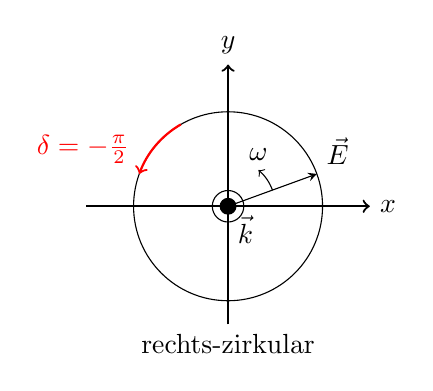
\begin{tikzpicture}[]
	% Achsen zeichnen
	\draw[->,thick] (-1.8,0) -- (1.8,0) node[right] {$x$};
	\draw[->,thick] (0,-1.5) -- (0,1.8) node[above] {$y$};
	%Plot
	%\draw[style=dashed] (-1.27,-1.05) rectangle (1.27,1.05);
	\draw (0, 0) circle (1.2);
	\draw (0, 0) circle (.2);
	\draw[fill=black] (0, 0) circle (.1);
	\draw (0,0) node[below right] {$\vec{k}$};
	\draw[->,>=stealth] (0,0)--(20:1.2) node[above right] {$\vec{E}$};
	\draw[->] (20:.6) arc (20:50:.6) node [above] {$\omega$};
	\draw [->,thick,color=red] (120:1.2) arc (120:160:1.2) node[above left] {$\delta = -\frac{\pi}{2}$};
	\draw (0,-1.5) node[below]{rechts-zirkular};
\end{tikzpicture}
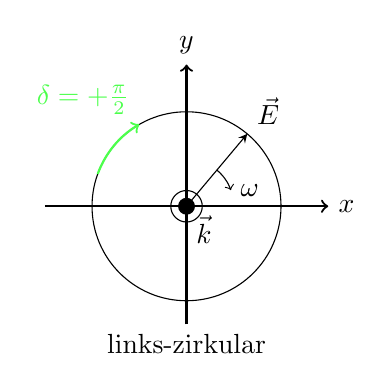
\begin{tikzpicture}[]
	% Achsen zeichnen
	\draw[->,thick] (-1.8,0) -- (1.8,0) node[right] {$x$};
	\draw[->,thick] (0,-1.5) -- (0,1.8) node[above] {$y$};
	%Plot
	%\draw[style=dashed] (-1.27,-1.05) rectangle (1.27,1.05);
	\draw (0, 0) circle (1.2);
	\draw (0, 0) circle (.2);
	\draw[fill=black] (0, 0) circle (.1);
	\draw (0,0) node[below right] {$\vec{k}$};
	\draw[->,>=stealth] (0,0)--(50:1.2) node[above right] {$\vec{E}$};
	\draw[->] (50:.6) arc (50:20:.6) node [right] {$\omega$};
	\draw [->,thick,color=green!70] (160:1.2) arc (160:120:1.2) node[above left] {$\delta = +\frac{\pi}{2}$};
	\draw (0,-1.5) node[below]{links-zirkular};
\end{tikzpicture}